	\section{Introduction}

\begin{frame}{I will present a method to solve PDE's on an unfitted mesh}
            % Column 1
    \begin{figure}
        \centering
        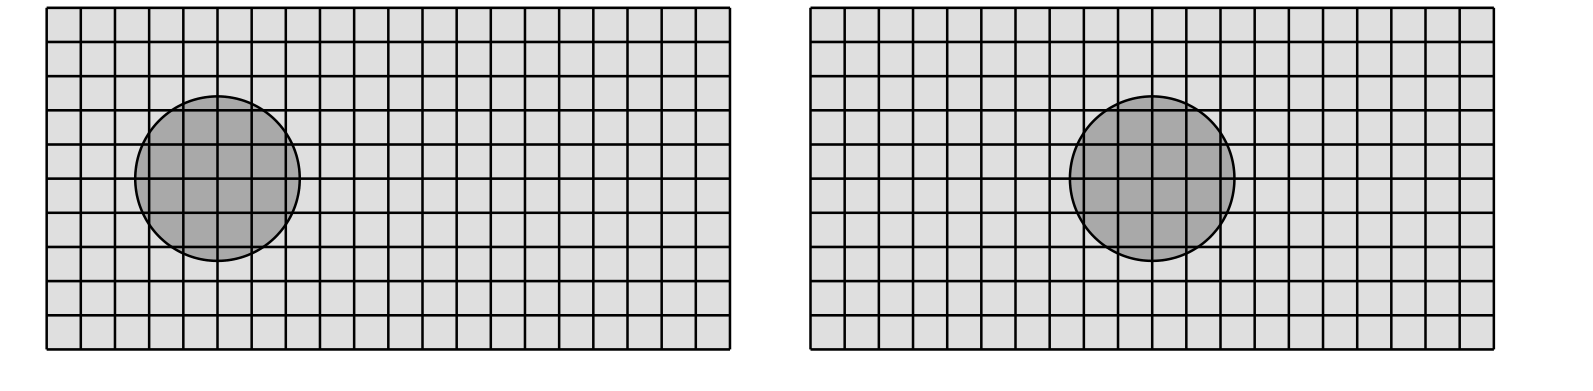
\includegraphics[width=10cm]{figures/transformed_mesh_unfitted.png}
    \end{figure}

    \begin{block}{}
        \begin{itemize}
            \item Fairly new class of methods! 5-10 years old.
            \item Can handle smooth boundaries and complex geometries!
            \item Possible to apply moving domains without re-meshing!
        \end{itemize}
    \end{block}
\end{frame}

    \begin{frame}{Maybe I should introduce myself}
        \begin{columns}
            % Column 1
            \begin{column}{0.5\textwidth}
                \begin{itemize}
                    \item Isak Hammer, 27 year old, Lofoten
                    \item Graduate student in Industrial Mathematics
                    \item Department of Mathematical Sciences (IMF)
                    \item Specialization in
                        \begin{enumerate}
                            \item Finite element methods
                                \begin{enumerate}
                                    \item Writing master thesis on unfitted methods for Cahn-Hilliard.
                                \end{enumerate}
                            \item Optimal control problems for PDEs
                                \begin{enumerate}
                                    \item Side projects on biomembrane dynamics
                                \end{enumerate}
                        \end{enumerate}
                    % \item Robotics engineer
                \end{itemize}
            \end{column}

            % Column 2
            \begin{column}{0.5\textwidth}
                \begin{figure}
                    \centering
                    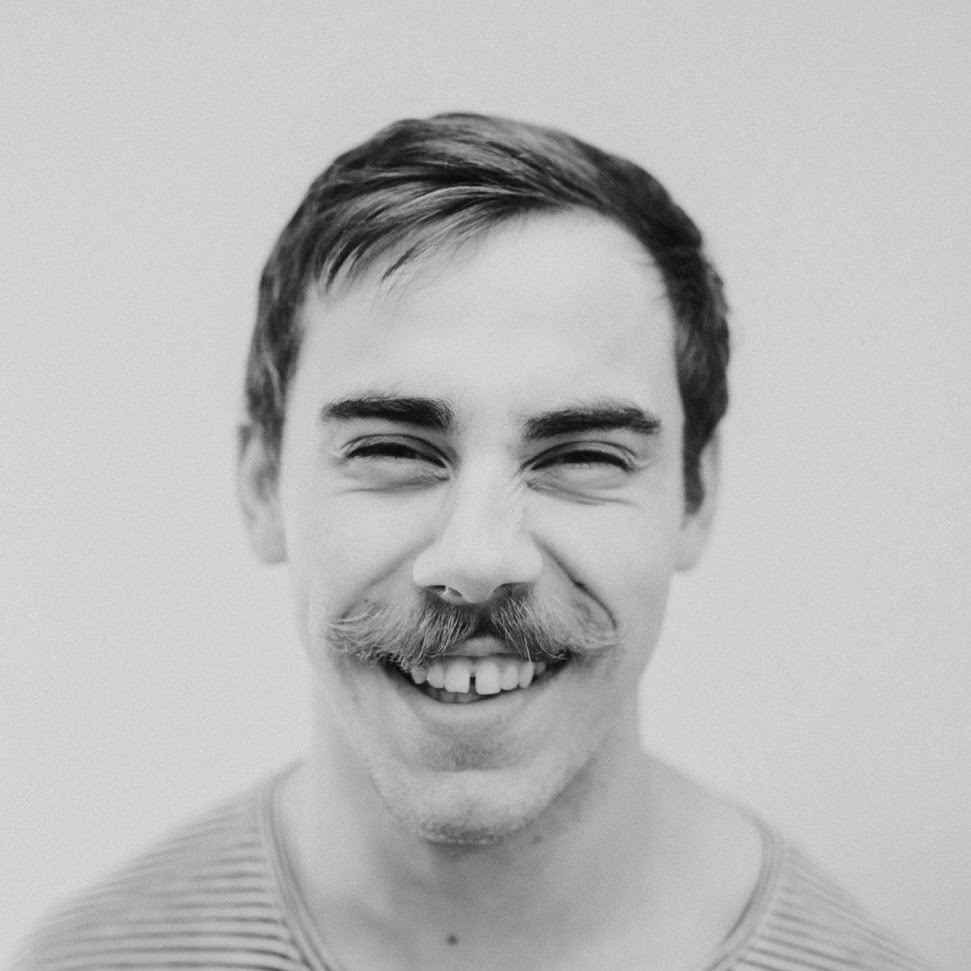
\includegraphics[width=0.7\textwidth]{figures/isak.jpg}
                \end{figure}
            \end{column}
        \end{columns}
    \end{frame}
\begin{frame}{Master student for one the CFD groups at IMF}
            % Column 1
    \begin{figure}
        \centering
        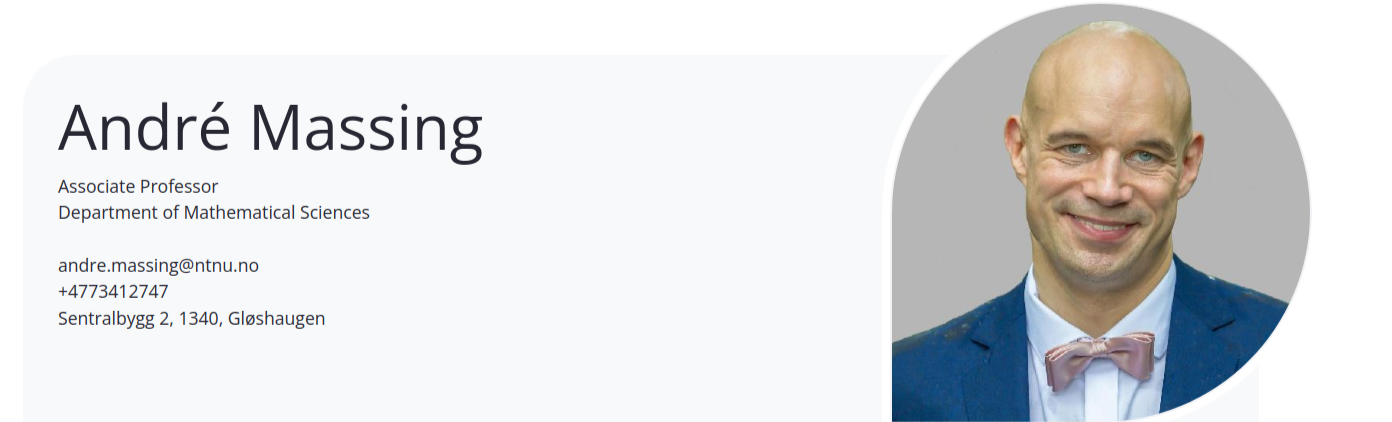
\includegraphics[width=10cm]{figures/AndreMassing.png}
    \end{figure}

    \begin{block}{}
        \begin{itemize}
            \item Research aligned towards biophysics problems
            \item $1 $ Postdoc
            \item $2 $ PhD candidates
            \item $1 $ Master's student
        \end{itemize}
    \end{block}
\end{frame}

    \begin{frame}{Introduction}
        \begin{columns}
            % Column 1
            \begin{column}{0.5\textwidth}
                \begin{itemize}
                    \item Offshore apprentice for 2 years
                    \item Worked with downhole electric instruments find reservoir properties
                        \begin{enumerate}
                            \item Reservoir permeability and pressure
                            \item Geological characteristics as rock dating, porosity etc.
                        \end{enumerate}
                \end{itemize}
            \end{column}

            % Column 2
            \begin{column}{0.5\textwidth}
                \begin{figure}
                    \centering
                    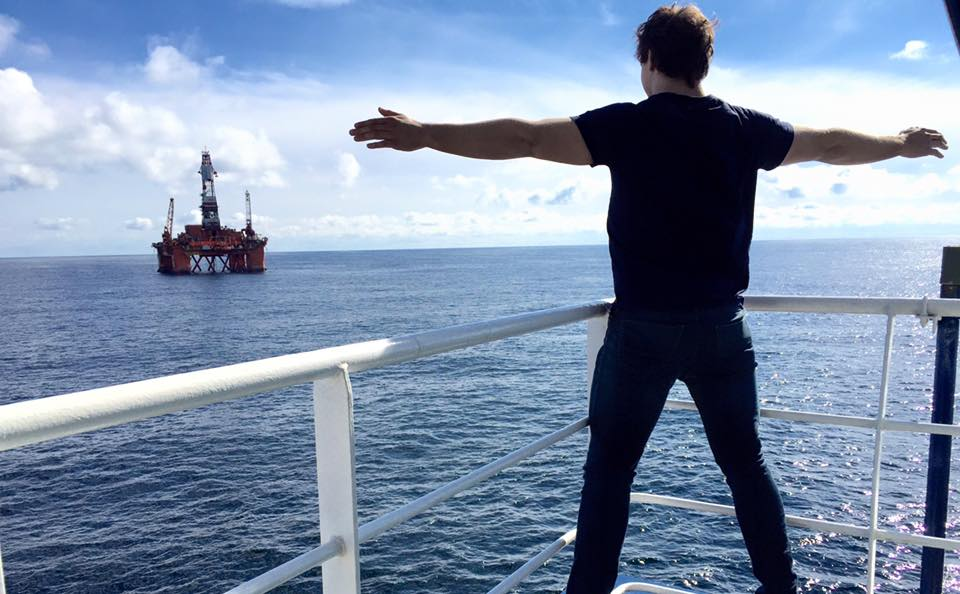
\includegraphics[width=1.0\textwidth]{figures/offshore.jpg}
                \end{figure}
            \end{column}
        \end{columns}
    \end{frame}



    \begin{frame}{Introduction}
        \begin{columns}
            % Column 1
            \begin{column}{0.5\textwidth}
                \begin{itemize}
                    \item Robotics Engineer for 2 years
                    \item  Revolve NTNU
                    \item Autonomous Systems
                        \begin{enumerate}
                            \item Vehicle Dynamics
                            \item Nonlinear MPC and trajectory optimization
                            \item Unknown path planning
                            \item Linux, C++, and Python \\
                             (Casadi, acados, ROS, Docker etc)
                        \end{enumerate}
                \end{itemize}
            \end{column}

            % Column 2
            \begin{column}{0.5\textwidth}
                \begin{figure}
                    \centering
                    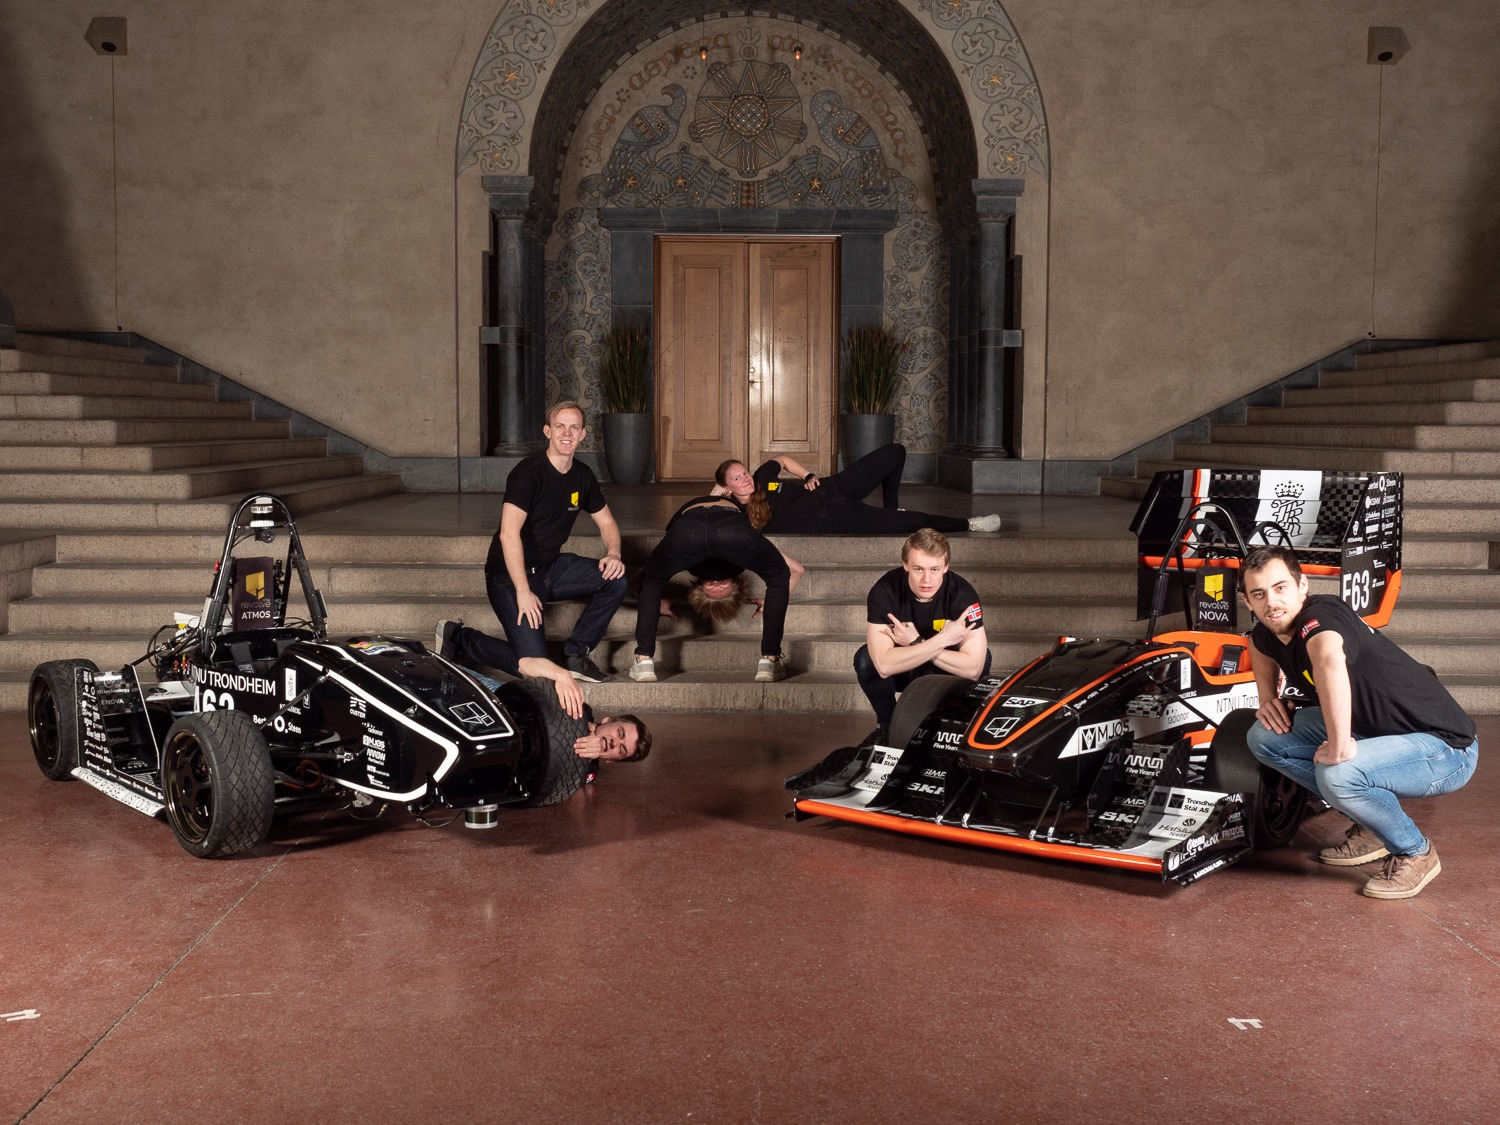
\includegraphics[width=1.0\textwidth]{figures/atmos.jpg}
                \end{figure}
            \end{column}
        \end{columns}
    \end{frame}

    \begin{frame}{Introduction}
            % Column 2
                \begin{figure}
                    \centering
                    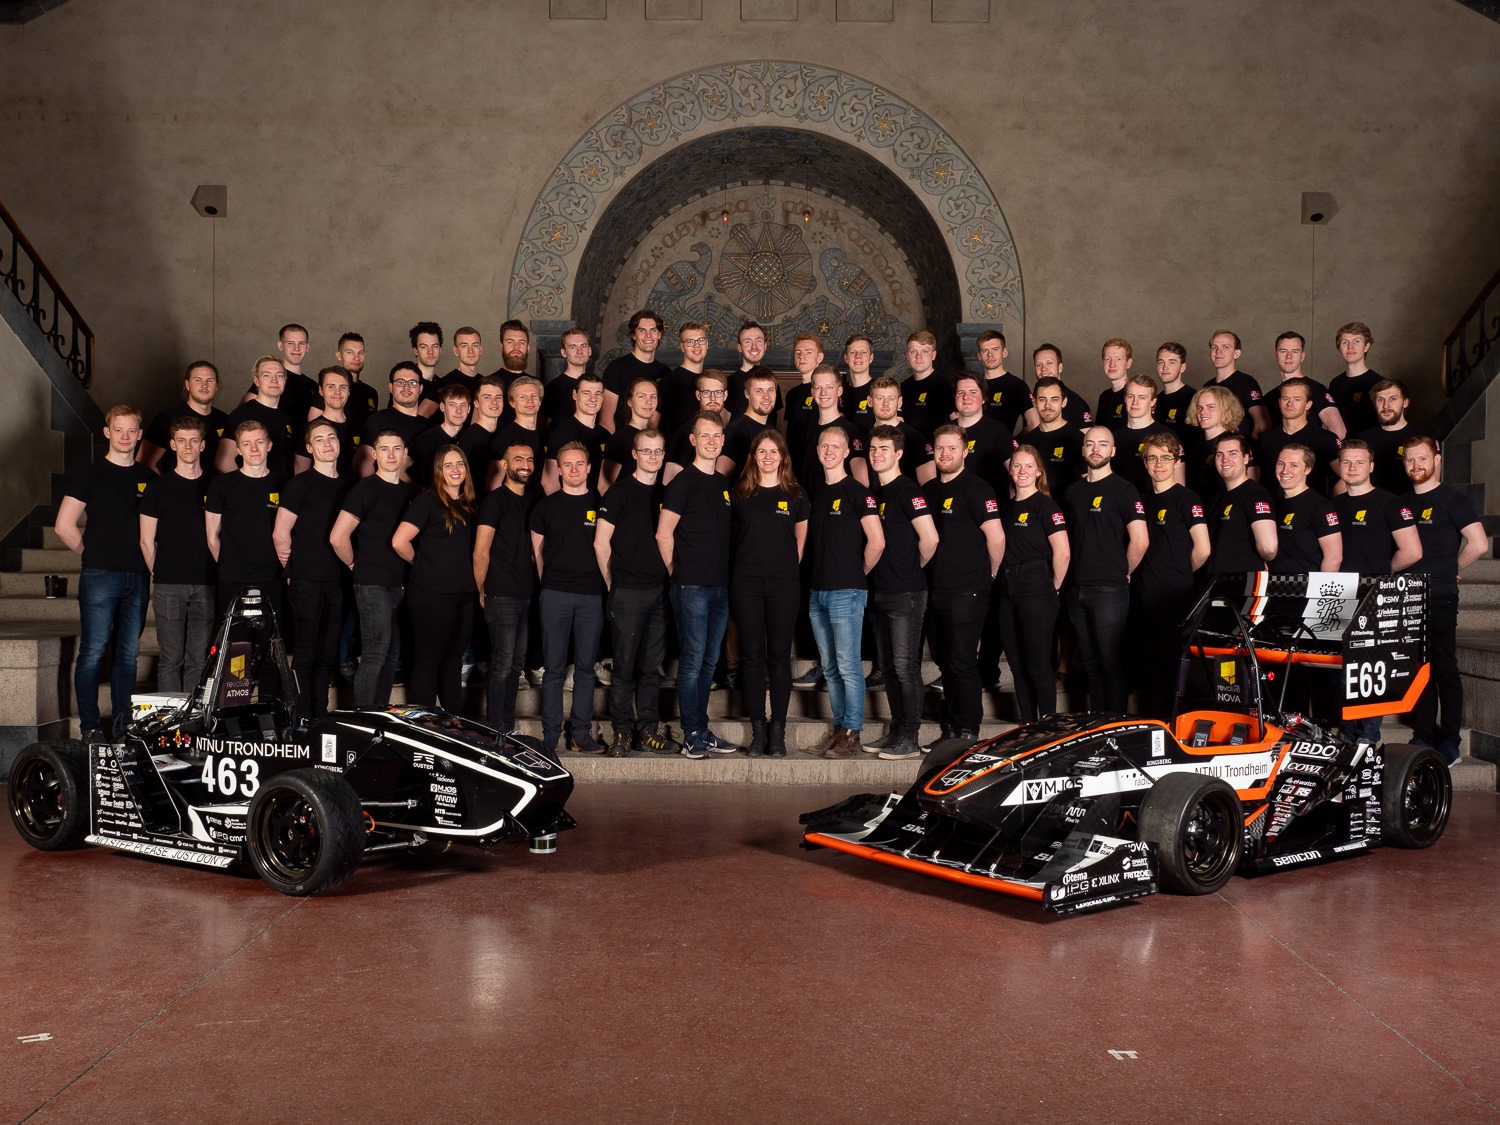
\includegraphics[width=0.65 \textwidth]{figures/revolve.jpg}
                \end{figure}
    \end{frame}

    \begin{frame}{Introduction}
                \begin{figure}
                    \centering
                    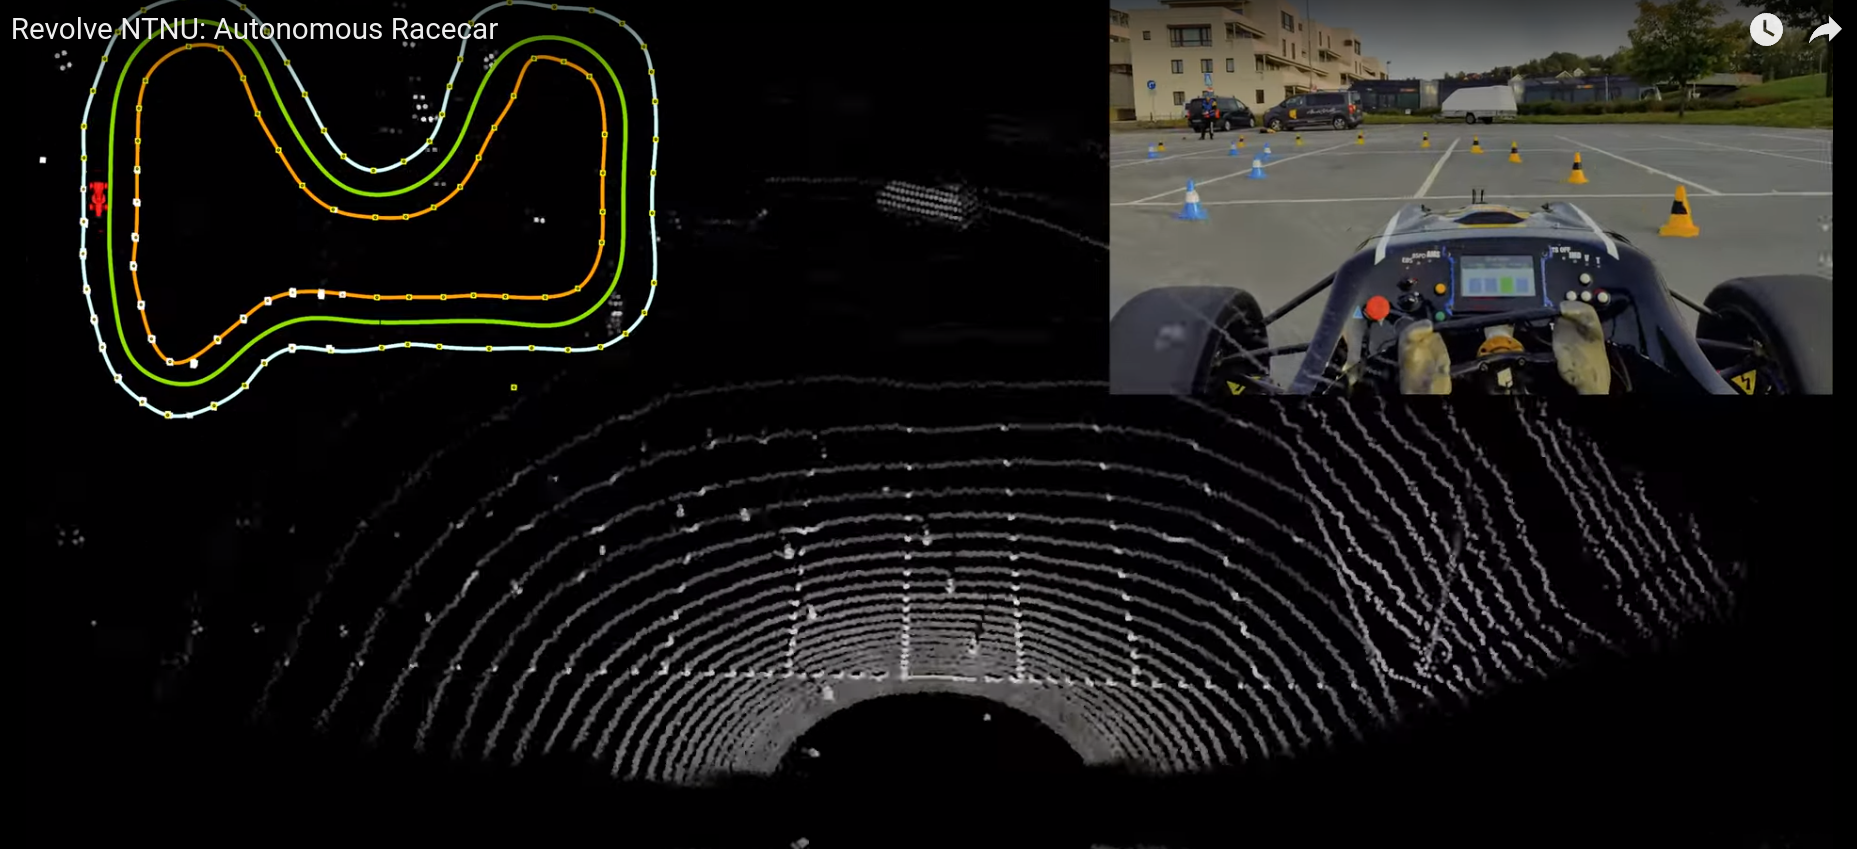
\includegraphics[width=0.90 \textwidth]{figures/revolve_video.png}
                \end{figure}
            Live demonstration of the system: \href{https://www.youtube.com/watch?v=_2T3MFnWG7A&t=44s&ab_channel=RevolveNTNU}{here}
    \end{frame}
